\documentclass[reqno,11pt]{amsart}
\usepackage{math327-lecture}
\usepackage{needspace}
\usepackage{tikz}
\usetikzlibrary{calc}
\newcommand{\Q}{\mathbb{Q}}
\newcommand{\C}{\mathbb{C}}
\lectureinfo{31}{Nov. 30, 2026}{Euclidean Domains, Prime and Irreducible Elements}
\artinsections{11.2; 12.2}

% Typeset from handwritten Lecture 33, Dec. 1, 2025, pp. 1--10.
\begin{document}
\raggedbottom
\makelecturetitle

\section{Integral domains}

\begin{define}[Integral domain]
A ring $R$ is an \emph{integral domain} (or simply a \emph{domain})
if whenever $ab=0$ in $R$, either $a=0$ or $b=0$.
If $ab=0$ with $a\neq0$ and $b\neq0$, then $a$ and $b$ are called
\emph{zero divisors}. Thus a domain is a ring without zero divisors.
\end{define}

A domain has the \emph{cancellation property}: if $ab=ac$ and
$a\neq0$, then $b=c$. Indeed, $a(b-c)=0$ and $a\neq0$ force
$b-c=0$.

We will study the following hierarchy of domains:
\[
  \{\text{Euclidean domains}\}\ \subseteq\
  \{\text{principal ideal domains}\}\ \subseteq\
  \{\text{unique factorization domains}\}.
\]

\begin{define}[Principal ideal domain]
A \emph{principal ideal domain} (PID) is a domain $R$ in which every
ideal $I\subseteq R$ has the form $I=(f)$ for some $f\in R$.
\end{define}

\section{Euclidean domains}

A Euclidean domain is a domain equipped with a size function that
allows division with remainder.

\begin{define}[Euclidean domain]
A \emph{Euclidean domain} is a domain $R$ together with a map
\[
  \sigma:R\setminus\{0\}\to\Z_{\geq0},
\]
called a \emph{size function}, with the following property:
if $a,b\in R$ and $a\neq0$, then there exist $q,r\in R$ such that
\[
  b=qa+r,
\]
where either $r=0$ or $\sigma(r)<\sigma(a)$.
\end{define}

\begin{remark}
The size function is just a map of sets; it is not a homomorphism.
\end{remark}

\begin{example}[Euclidean domains]\leavevmode
\begin{itemize}
  \item $\Z$, with $\sigma(m)=|m|$.
  \item $\Q[x]$, with $\sigma(f)=\deg f$.
  \item $\Z[i]$, the ring of \emph{Gaussian integers}, with
  \[
    \sigma(\alpha)=|\alpha|^2=m^2+n^2\qquad\text{for }\alpha=m+ni.
  \]
\end{itemize}
\end{example}

\Needspace{14\baselineskip}
\begin{example}[Division with remainder in $\Z{[i]}$]
Fix a nonzero $\alpha\in\Z[i]$, for instance $\alpha=2+i$.
The principal ideal $(\alpha)$ consists of the multiples $z\alpha$
with $z=m+ni\in\Z[i]$. Writing $\alpha=re^{i\theta}$ and
$z=se^{i\varphi}$, we have
\[
  z\alpha=sr\,e^{i(\theta+\varphi)},
\]
so multiplication by $\alpha$ rotates by $\theta$ and scales by
$|\alpha|=r$. It carries the unit square with vertices
$0,1,i,1+i$ to a square of side $|\alpha|$; for $\alpha=2+i$,
the vertex $1$ goes to $2+i$ and the vertex $i$ goes to
$(2+i)i=-1+2i$. Hence the multiples of $\alpha$ form a square
lattice of side length $|\alpha|$, tiling the plane by squares.

\begin{center}
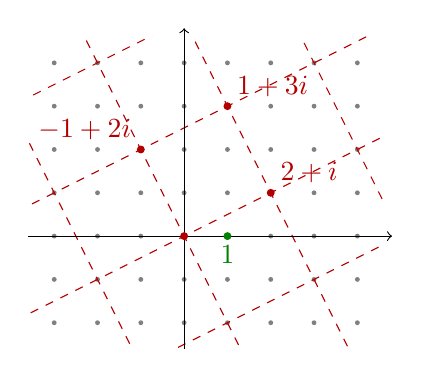
\begin{tikzpicture}[scale=0.55]
  \begin{scope}
    \clip (-3.6,-2.6) rectangle (4.6,4.6);
    \foreach \x in {-3,...,4} \foreach \y in {-2,...,4}
      {\fill[gray] (\x,\y) circle (1.6pt);}
    \foreach \n in {-4,...,4}
      {\draw[dashed,red!70!black] ($(-8,-4)+\n*(-1,2)$) -- ($(8,4)+\n*(-1,2)$);}
    \foreach \m in {-4,...,4}
      {\draw[dashed,red!70!black] ($(4,-8)+\m*(2,1)$) -- ($(-4,8)+\m*(2,1)$);}
  \end{scope}
  \draw[->] (-3.6,0) -- (4.8,0);
  \draw[->] (0,-2.6) -- (0,4.8);
  \fill[red!70!black] (2,1) circle (2.6pt) node[above right] {$2+i$};
  \fill[red!70!black] (-1,2) circle (2.6pt) node[above left] {$-1+2i$};
  \fill[red!70!black] (1,3) circle (2.6pt) node[above right] {$1+3i$};
  \fill[red!70!black] (0,0) circle (2.6pt);
  \fill[green!50!black] (1,0) circle (2.6pt) node[below] {$1$};
\end{tikzpicture}
\end{center}

Every point of the plane lies in one of these squares, and its
distance to the nearest vertex of that square is at most half
the diagonal,
\[
  d=\tfrac12\sqrt{|\alpha|^2+|\alpha|^2}=\frac{|\alpha|}{\sqrt2},
  \qquad\text{so}\qquad d^2<|\alpha|^2.
\]
Therefore, given any $\beta\in\Z[i]$, we can find $q\in\Z[i]$ such
that $q\alpha$ is a vertex of a square containing $\beta$ nearest to
$\beta$, and then
\[
  |\beta-q\alpha|^2\leq d^2<|\alpha|^2=\sigma(\alpha).
\]
% NOTE: notes write |beta - q alpha| < |alpha|^2; the intended
% (and needed) inequality is |beta - q alpha|^2 < |alpha|^2.
Setting $r=\beta-q\alpha$, we get $\beta=q\alpha+r$ with $r=0$ or
$\sigma(r)<\sigma(\alpha)$. So $\Z[i]$ is a Euclidean domain.
\end{example}

\section{Euclidean domains are principal ideal domains}

\begin{theorem}\label{thm:ed-pid}
Every Euclidean domain is a principal ideal domain.
\end{theorem}
\begin{proof}
The argument follows what we did for $\Z$ and $\Q[x]$.
Let $R$ be a Euclidean domain with size function $\sigma$, and let
$I\subseteq R$ be an ideal. We want to find $f\in I$ such that
$I=(f)$. If $I=(0)$, take $f=0$, so assume $I\neq(0)$.

For each nonzero $x\in I$, consider $\sigma(x)\in\Z_{\geq0}$.
Pick a smallest element of the nonempty set
\[
  \sigma(I)=\{\sigma(x):x\in I\setminus\{0\}\},
\]
and let $f\in I\setminus\{0\}$ be an element attaining it.
Clearly $(f)\subseteq I$. To show $I=(f)$, pick $a\in I$ and write
\[
  a=qf+r,\qquad r=0\text{ or }\sigma(r)<\sigma(f).
\]
Since $I$ is an ideal, $r=a-qf\in I$. If $r\neq0$, then
$\sigma(a-qf)<\sigma(f)$ contradicts the minimality of
$\sigma(f)$. Hence $r=0$ and $a=qf\in(f)$.
\end{proof}

\begin{remark}
The inclusion of Euclidean domains in PIDs is strict. For example,
\[
  \Z\Bigl[\tfrac12\bigl(1+\sqrt{-19}\bigr)\Bigr]
\]
is a PID but not a Euclidean domain. The proof is elementary but
long; a separate write-up explaining it is posted on Canvas.
\end{remark}

So far we have
\[
  \text{E.D.}\ \subsetneq\ \text{PID}\ \subseteq\ \text{UFD}.
\]
What is a UFD?

\section{Units, associates, and uniqueness of factorization}

In $\Z$, we have $(d)\subseteq(p)$ if and only if $p\mid d$.
Every nonzero integer $n\neq\pm1$ factors into primes,
\[
  n=\pm p_1\cdots p_r=\pm p_1^{a_1}\cdots p_\ell^{a_\ell},
\]
but what does it mean to be prime? Already in $\Z$ there are
choices of sign:
\[
  -18=-3^2\cdot2=(-3)^2\cdot(-2).
\]
% NOTE: the notes write "18 = (-3)^2 (-2)"; corrected to -18.

\begin{define}[Units and associates]
The \emph{units} of a ring $R$ are the elements of $R$ having
multiplicative inverses; they form a group $R^\times$. Elements
$a,b\in R$ are \emph{associates} if
\[
  a=bu\qquad\text{for some }u\in R^\times,
\]
and we then write $a\sim b$.
\end{define}

\begin{example}
We have $\Z^\times=\{\pm1\}$, so in $\Z$ we have $n\sim-n$.
\end{example}

``Uniqueness'' of factorization in $R$ should mean the following:
if
\[
  a=p_1\cdots p_r=q_1\cdots q_s,
\]
then $r=s$ and, after rearranging, $p_i\sim q_i$ for each $i$.
For instance, $18=3\cdot3\cdot2=(-3)\cdot(-3)\cdot2$ are the
same factorization in this sense.

\begin{example}[Gaussian integers]
We have $\Z[i]^\times=\{\pm1,\pm i\}$, and
\[
  (2+i)(2-i)=5=(1+2i)(1-2i).
\]
These are the same factorization, since
\[
  2+i=i(1-2i)\sim1-2i,\qquad 2-i=-i(1+2i)\sim1+2i.
\]
% NOTE: the notes pair 2+i ~ 1+2i and 2-i ~ 1-2i, which is false
% ((1+2i)/(2+i) = (4+3i)/5 is not a Gaussian integer); the correct
% pairing is 2+i ~ 1-2i and 2-i ~ 1+2i.
\end{example}

\section{Irreducible and prime elements}

There are two natural notions of ``prime''. If $p$ is a prime
number, then:
\begin{itemize}
  \item we cannot break $p$ up further: if $p=ab$ with $a,b$
  positive, then $a=1$ or $b=1$;
  \item if $p\mid ab$, then $p\mid a$ or $p\mid b$.
\end{itemize}

\begin{define}[Irreducible and prime elements]
Let $R$ be a ring, and let $a,p\in R$ be nonzero nonunits.
% NOTE: "nonzero nonunit" is not written in the notes but is the
% standard hypothesis in both definitions.
\begin{itemize}
  \item $a$ is \emph{irreducible} if whenever $a=bc$, either $b$ or
  $c$ is a unit.
  \item $p$ is a \emph{prime element} if whenever $p\mid ab$,
  either $p\mid a$ or $p\mid b$.
\end{itemize}
\end{define}

\begin{lemma}\label{lem:prime-irred}
If $R$ is a domain, then every prime element of $R$ is irreducible.
\end{lemma}
\begin{proof}
Assume $p$ is prime; we show that it is irreducible. Suppose $p=ab$.
Then $p\mid ab$, so $p\mid a$ or $p\mid b$; say $p\mid a$, so that
$a=px$ for some $x\in R$. Then
\[
  p=ab=pxb.
\]
Since $p\neq0$, cancellation gives $1=xb$, so $b$ is a unit.
\end{proof}

In a PID the converse also holds: irreducible elements are prime.

\begin{theorem}\label{thm:pid-irred-prime}
In a principal ideal domain, an element is prime if and only if it
is irreducible.
\end{theorem}

\end{document}
